\section{Probabilistic Model}
\label{sec:model}


\newcommand{\pattern}{\mathcal{P}}
\newcommand{\group}{g}
\newcommand{\groups}{\mathcal{G}}
\newcommand{\segment}{s}
\newcommand{\segments}{\mathcal{S}}
\newcommand{\model}{\mathcal{M}}
\newcommand{\term}{\mathcal{T}}
\newcommand{\weights}{\mathbf{w}}
\newcommand{\dataset}{\mathcal{D}}
\newcommand{\variable}[1]{\mathbf{#1}}
\newcommand{\colorVars}{\variable{C}}
\newcommand{\colors}{\variable{c}}
\newcommand{\features}{\variable{f}}
\newcommand{\termStats}{\Phi_\term}
\newcommand{\termInstStats}{\phi_\term}
\newcommand{\expectation}{\mathds{E}}

\newcommand{\prop}{\pi}
\newcommand{\unaryProps}{\Pi^{\textrm{Unary}}}
\newcommand{\binaryProps}{\Pi^{\textrm{Binary}}}
\newcommand{\groupTerm}{\Phi^{\textrm{Grp}}_\pi}
\newcommand{\segTerm}{\Phi^{\textrm{Seg}}_\pi}
\newcommand{\adjTerm}{\Phi^{\textrm{Adj}}_\pi}
\newcommand{\neighbors}{n}
\newcommand{\adj}{\text{adj}}
\newcommand{\adjStrength}{\text{str}}
\newcommand{\size}{A}
\newcommand{\groupInstStats}{\phi^{\textrm{Grp}}_\pi}
\newcommand{\segInstStats}{\phi^{\textrm{Seg}}_\pi}
\newcommand{\adjInstStats}{\phi^{\textrm{Adj}}_\pi}
\newcommand{\groupTermWeight}{\mathbf{w}^{\textrm{Grp}}_\pi}
\newcommand{\segTermWeight}{\mathbf{w}^{\textrm{Seg}}_\pi}
\newcommand{\adjTermWeight}{\mathbf{w}^{\textrm{Adj}}_\pi}
\newcommand{\colorCompatWeight}{\mathbf{w}^{\textrm{ColorCompat}}_\pi}

\newcommand{\colorCompatTerm}{\Phi^{\textrm{ColorCompat}}}
\newcommand{\factor}{\mathcal{F}}
\newcommand{\segprime}{\segment^{\prime}}
\newcommand{\groupprime}{\group^{\prime}}

\newcommand{\propName}[1]{\text{\emph{#1}}}


% Notational conventions:

% Our model: $\model$. A term in our model: $\term$. The vector of weights for the entire model: $\weights$. The weight for a particular term: $\weights_\term$.

% A pattern template: $\pattern = (\segments, \groups, \colorVars, \features)$, where $\groups$ is a set of individual groups $\group$, $\segments$ is a set of individual segments $\segment$, $\colorVars$ is a set of color variables, and $\features$ is a set of features.

% The color variable of a group: $\colorVars(\group)$. The color variable of a segment: $\colorVars(\segment)$.

% An assignment of colors to color variables: $\colors$.

% The features of a segment: $\features(\segment)$. The features of a group: $\features(\group)$. The features of a pair of segments: $\features(\segment_1, \segment_2)$.

% A training dataset: $\dataset$. An example from a training dataset: $(\pattern, \colors)$.

% Sufficient statistics for a term in our model: $\termStats$.

% The probability distribution encoded by our model:
% \begin{equation*}
% p(\colors | \pattern : \weights) = \frac{1}{Z_\pattern(\weights)} \prod_{\term \in \model} \exp{\frac{ \weights_\term \cdot \termStats(\colors, \pattern)}{t}}
% \end{equation*}

% Statistics for group terms:
% \begin{equation*}
% \groupTerm(\colors, \pattern) = \sum_{\group \in \groups_\pattern} \ln p( \prop( \colors(\group) ) | \features_\pattern(\group)) \cdot \size_\group
% \end{equation*}

% Statistics for segment terms:
% \begin{equation*}
% \segTerm(\colors, \pattern) = \sum_{\segment \in \segments_\pattern} \ln p( \prop( \colors(\segment) ) | \features_\pattern(\segment)) \cdot \size_\segment
% \end{equation*}

% Statistics for adjacency terms:
% \begin{equation*}
% \newcommand{\segprime}{\segment^{\prime}}
% \adjTerm(\colors, \pattern) =
% 	\sum_{(\segment, \segprime) \in \adj(\pattern)}
% 		\ln p( \prop( \colors(\segment), \colors(\segprime) ) | \features_\pattern(\segment, \segprime) ) \cdot \adjStrength(\segment, \segprime) 
% \end{equation*}

%\remark{In every subsection, motivate why this particular term is needed. Briefly relate to any relevant algorithmic details from previous work.}

%To be safe, temporarily separating out the spatial arrangement and color compatibility subsection

We formulate the problem of generating colorings for a pattern template as finding high-probability colorings under a probabilistic model. Formally, we define a pattern template as $\pattern = (\groups, \segments, \colorVars, \features)$, where $\groups$ is a set of individual groups $\group$, $\segments$ is a set of individual segments $\segment$, $\colorVars$ is a set of color variables, and $\features$ is a set of features over different groups, segments, and segment adjacencies within the pattern. Each group $\group$ and segment $\segment$ is associated with a color variable ($\colorVars_\group$ and $\colorVars_\segment$, respectively). All segments within a color group have the same color by definition, so $\colorVars_{\text{group}(\segment)} = \colorVars_\segment$. A coloring $\colors$ is an assignment of colors to color variables.

We define the probability of a coloring for a particular pattern template as a log-linear model:  
\begin{equation*}
 p(\colors | \pattern : \weights) = \frac{1}{Z_\pattern(\weights)} \prod_{\term \in \model} \exp(\termWeight \cdot \termStats(\colors, \pattern))
\end{equation*}
The model $\model$ is comprised of a number of different terms $\term$, where each term scores the goodness of a color assignment based on a term-dependent statistic $\termStats(\colors,\pattern)$. $Z_\pattern(\weights)$ is the pattern-dependent partition function that normalizes the distribution. Each term also has a weight $\termWeight$ which determines its relative contribution to the model; the method used for setting these weights is detailed in Section~\ref{sec:weights}. Bolded symbols are vector-valued while non-bolded symbols are scalar.

This type of model is well-suited to the coloring-generation problem. It is very flexible; in principle, the individual term statistics $\termStats$ can be any real-valued function. In our model, we include terms both for color compatibility as well as for spatial properties defined over groups, segments, and segment adjacencies. Users can also guide the model via additional soft constraint terms (Section~\ref{sec:results}). In addition, it is very easy to compare the relative importance of each term by comparing their weights, which we will do in Section~\ref{sec:weights} to gain some insight into which terms contribute the most to producing attractive colorings. 

The model can also be interpreted graphically as a factor graph (Yeh et al.~\shortcite{YiTingTiledPatterns} provides an accessible introduction for the graphics community). Each type of term contributes different factors $\factor$ to the graph. For example, our color compatibility term contributes a factor over at most five color variables that scores the compatibility of those colors. The spatial terms contribute a unary factor for each color variable and binary factors for color variables that are adjacent in the pattern. Figure~\ref{fig:FactorGraph} shows an example of such a factor graph. Circles denote the color variables, while squares denote the different factors $\factor$, and edges connect each factor to the variables within their scope. 


\begin{figure}[ht]
\begin{tabular}{cc}
\raisebox{4em}{
\includegraphics[width=.2\columnwidth]{figs/factorGraphPattern}} &
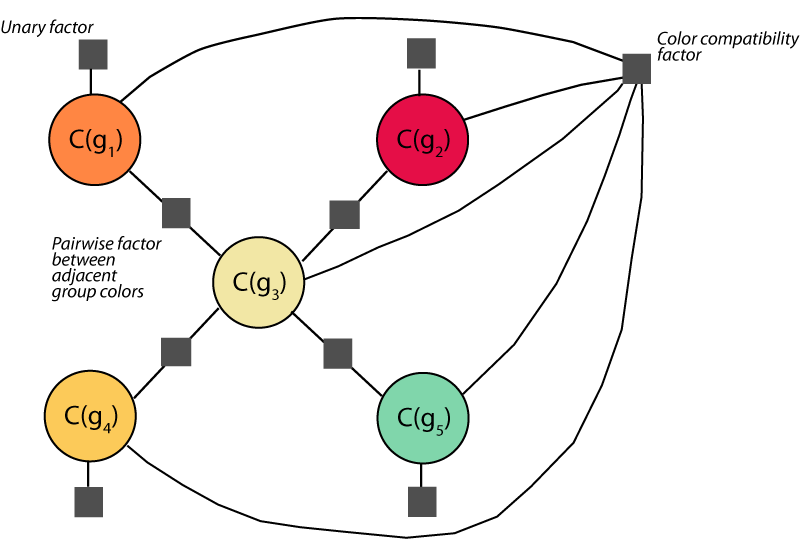
\includegraphics[width=.7\columnwidth]{figs/factorGraph} \\
\end{tabular} 
\caption{A factor graph for an example pattern template. Factors correspond with the color compatibility and spatial terms from our model. In the figure, nodes are colored according to their corresponding color group in the pattern\remark{Rough figure.}}
\label{fig:FactorGraph}
\end{figure}



\subsection{Color Compatibility}
\label{sec:colorCompat}

Previous work has shown that the aesthetic appeal of an image can be improved by increasing the compatibility or harmony of image colors ~\cite{CohenOrHarmonization,DressUp,ColorizationUsingHarmony,ODonovan}. Our model includes a color compatibility term to score the general appeal of the colors in an assignment, based on the compatibility model introduced by O'Donovan et al.~\shortcite{ODonovan}. This compatibility model predicts 0-5 numeric aesthetic ratings for five-color `color themes,' which are ordered rows of five colors. 

We extract such a color theme from a pattern by taking the colors of the five largest color groups and ordering them by size. If the pattern contains fewer than five color groups, we repeat colors in order of size to fill the rest of the theme. Inspection of five-color patterns showed that size-ordering of colors tends to produce themes that are, on average, rated higher than random orderings but lower than the optimal ordering. Additionally, ordering has little effect on discriminative power: in general, low-scoring themes are rated lower than high-scoring themes regardless of permutation.

The term statistic is then defined as the log-normalized theme rating under O'Donovan's compatibility model:
\begin{equation*}
\colorCompatTerm(\colors| \pattern) = \ln(compat(theme(\colors| \pattern))/5)
\end{equation*}
where $\textsl{theme}$ is the ordered theme extracted from the pattern and $\textsl{compat}$ is the predicted rating from the O'Donovan model.

Here we use the O'Donovan model of color compatibility. However, the model is flexible and can accomodate any other color compatibility or harmony model that can score a set of colors.

In the factor graph representation of our model, this term contributes one factor that touches the five color variables belong to the five largest groups (or fewer, if there are less than five groups in the pattern):
\begin{equation*}
\factor(\textrm{top}(\colorVars) | \pattern) = \exp(\colorCompatWeight \cdot \colorCompatTerm(\colorVars | \pattern))
\end{equation*}
where $\textsl{top}$ are the color variables of the largest five groups in the pattern.


\subsection{Spatial Properties}
\label{sec:spatialCompat}

As shown in Figure~\ref{fig:ColorCompatOnly}, color compatibility alone does not predict attractive colorings. Good color assignments also depend on the properties of the regions being colored and their spatial arrangement. To capture these dependencies, our model includes spatial terms over groups, segments, and segment adjacencies in the pattern. Group and segment terms capture color dependencies on region features, and segment adjacency terms capture color dependencies on the relationship between nearby regions.

These spatial terms score color assignments based on the conditional probability of a color property $\prop$ (such as lightness or colorfulness) given the features of an object $x$ (which is either a group, segment, or segment adjacency). We compute these probabilities on color properties instead of directly on colors to allow for more generalization over colors that do not occur in the model's training data.
%%%
%\begin{align*}
%	\termStats(\colors | \pattern) &= \sum_{x \in \pattern} \termInstStats(\colors_x | \pattern, x) \\
%	%\termInstStats(x, \colors| \pattern) &= \ln p(\prop(\colors(x)) | \features(x)) \cdot s_x
%	\termInstStats(\colors_x | \pattern, x) &\propto p(\prop(\colors_x) | \features_x)
%\end{align*}
%%%
%\remark{Yes, these are correct, but they seem redundant or at least confusing. When you go on to read the equation in the next subsection, you spend a lot of time trying to match terms back to this equation and the correspondences are weird.}
For example, Figure~\ref{fig:conditionalDistribution} shows the conditional probability distribution over lightness for the background group of one pattern. The distribution is conditional on several characteristic features of the group, such as its size and the number of segments it contains. In the next sections, we give definitions for the group and segment terms in the model (Section~\ref{sec:groupAndSegTerms}) and the adjacency terms (Section~\ref{sec:adjTerms}). We then describe how to learn these conditional probability distributions from example patterns (Section~\ref{sec:learningPdfs}). A complete listing of the features used, as well as more details on the computation of color properties, can be found in the Appendix.

\begin{figure}[ht]
\begin{tabular}{cc}
\raisebox{5em}{
\includegraphics[width=.22\columnwidth]{figs/histogramImage}}&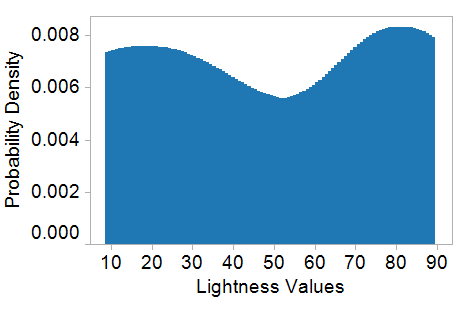
\includegraphics[width=.7\columnwidth]{figs/histogram}%\vspace{0.5em}\\
\end{tabular}
\caption{The conditional probability distribution of lightness values for the background color group of a pattern (highlighted in orange). The distribution's multimodality indicates that either very light or very dark backgrounds may be acceptable for this pattern.}
\label{fig:conditionalDistribution}
\end{figure}

\subsubsection{Group and Segment Terms}
\label{sec:groupAndSegTerms}

Both global group features as well as local segment features affect the appearance of a color assignment. The total area of a group and overall spread of its member segments correspond to the overall proportion and spread of its assigned color within an image. In addition, the size and shape of member segments may impact the color a group takes on. As an example, smaller segments may often be more saturated, and a group composed of many small segments may be more likely to be saturated than a group composed of a few small segments but also one large segment \remark{S: Made up example. Should probably find one that holds in our data}.

Our model has one group and one segment term for each of the color properties $ \prop \in \unaryProps$, which are \propName{Lightness}, \propName{Colorfulness}, \propName{NameCounts}, and \propName{NameSaliency}.
The properties \propName{Lightness} and \propName{Colorfulness} are computed in \lab space. \propName{NameCounts} (counts of how many times a color is described with different names) and \propName{NameSaliency} (how uniquely a color is named) are as described by Heer and Stone~\shortcite{ColorNamingModels}. While lightness and colorfulness capture perceptual properties of color, name saliency and color name counts capture more categorical properties.

The group term for property $\prop \in \unaryProps$ has the statistic:
\begin{align*}
 \groupTerm(\colors|\pattern) &= \sum_{\group \in \groups} \groupInstStats(\colors_\group | \pattern, \group) \\
 \groupInstStats(\colors_\group | \pattern, \group) &=  \ln p( \prop( \colors_\group ) | \features_\group ) \cdot \size_\group
\end{align*}
where $\size_\group$ is the area of the group $\group$ and $\features_\group$ are the features of the group $\group$ (See the Appendix for the complete list of features used). We weight the contribution of each group to the term statistics by its relative area as larger regions tend to have more impact on the appearance of a coloring.

Similarly, the segment term for property $\prop$ has the statistics function $\segTerm(\colors|\pattern) = \sum_{\segment \in \segments} \segInstStats(\colors_\segment | \pattern, \segment)$, where $\segInstStats(\colors_\segment | \pattern, \segment) = \ln p( \prop( \colors_\segment ) | \features_\segment) \cdot \size_\segment$. Here, $\size_\segment$ is the size of the segment $\segment$ and $\features_\segment$ are the features of $\segment$.

%Similarly, the segment term for property $\prop$ has the statistics function:
%\begin{align*}
% \segTerm(\colors|\pattern) = \sum_{\segment \in \segments} \segInstStats(\colors_\segment | \pattern, \segment) \\
% \segInstStats(\colors_\segment | \pattern, \segment) = \ln p( \prop( \colors_\segment ) | \features_\segment) \cdot \size_\segment
%\end{align*}
%
%\remark{Is there much to be gained by not inlining directly? This equation is already pretty redundant with the previous one, just replacing groups for segments.}
%
%where $\size_\segment$ is the size of the segment $\segment$ and $\features_\segment$ are the features of $\segment$.

These terms contribute unary factors over each color variable by grouping together statistics for the group and segments associated with the variable:
\begin{align*}
 %\factor(\colorVars(\group)) = \prod_{\prop \in \unaryProps} \exp\left(\frac{\groupTermWeight \cdot \groupInstStats(\group) + \segTermWeight \cdot \sum_{\segment \in \group} \segInstStats(\segment)}{t}\right) 
 \factor(\colorVars_\group | \pattern) = \prod_{\prop \in \unaryProps}
 		\exp( (&\groupTermWeight \cdot \groupInstStats(\colorVars_\group | \pattern, \group)  \\
 		     + &\segTermWeight \cdot \sum_{\segment \in \group} \segInstStats(\colorVars_\group | \pattern, \segment))) 
\end{align*}


\subsubsection{Segment Adjacency Terms}
\label{sec:adjTerms}

While group and segment terms model the dependency of color assignments on features of same-color regions, they do not capture relationships between different-color regions. In particular, adjacent color regions can have strong effects on their neighbor's perceived color, making colors seem more or less saturated or causing vibrating boundaries if adjacent lightness and colorfulness are too similar~\cite{AlbersInteractionOfColor}. Thus, we also add segment adjacency terms to the model.

Good color assignments to adjacent segments may depend on the nature of their adjacency. For example, a square enclosed by a thin border appears different from a square enclosed by a thick border, and different again from a square side-by-side with another square (Figure~\ref{fig:surround}). Thus, when computing features of an adjacency we include the features of the segments involved as well as how much one neighbor encloses another.
\begin{figure}[ht]
\centering

\includegraphics[width=.7\columnwidth]{figs/surround}
\caption{Color appearance depends on relationships with surrounding regions\remark{Rough figure.}}
\label{fig:surround}
\end{figure}



%~\remark{D: These examples might work better with pictures...} 

Our model has one adjacency term for each of the color properties $ \prop \in \binaryProps$, which are \propName{RelativeLightness}, \propName{RelativeColorfulness}, \propName{PerceptualDifference}, \propName{ChromaDifference}, and \propName{NameSimilarity}.
As with group and segment terms, \propName{RelativeLightness} and \propName{RelativeColorfulness} are computed in \lab space. \propName{PerceptualDifference} is Euclidean distance in \lab space, and \propName{ChromaDifference} is the percentage of that distance that is due to the chroma channels. Finally, \propName{NameSimilarity} is the color name cosine similarity measure defined by Heer and Stone~\shortcite{ColorNamingModels}.

The sufficient statistics function for each binary property is:
 \begin{align*}
 \adjTerm(\colors | \pattern) &= \sum_{(\segment, \segprime) \in \adj(\pattern)} \adjInstStats(\colors_\segment, \colors_\segprime | \pattern, \segment, \segprime) \\
 \adjInstStats(\colors_\segment, \colors_\segprime | \pattern, \segment, \segprime) &= \ln p( \prop( \colors_\segment, \colors_\segprime ) | \features_{\segment, \segprime} ) \cdot \adjStrength(\segment, \segprime)
\end{align*}
where $\adjStrength(\segment,\segprime)$ is the strength of the adjacency $(\segment,\segprime)$. We define adjacency strength as the number of pixels from segments $\segment$ or $\segprime$ that are within a 2-pixel distance from their perimeters. All adjacency strengths are normalized to sum to 1.  

These terms contribute binary factors over each adjacent pair of color variables:
\begin{equation*}
 %\factor(\colorVars(\group), \colorVars(\groupprime)) = \prod_{\prop \in \binaryProps} \exp\left(\frac{\adjTermWeight \cdot \sum_{(\segment, \segprime) \in \adj(\group, \groupprime)} \adjInstStats(\segment, \segprime)}{t}\right) 
 \factor(\colorVars_\group, \colorVars_\groupprime | \pattern) = \prod_{\prop \in \binaryProps} \exp( (\adjTermWeight \cdot \sum_{\mathclap{(\segment, \segprime) \in \adj(\group, \groupprime)}} \adjInstStats( \colorVars_\group, \colorVars_\groupprime | \pattern, \segment, \segprime))) 
\end{equation*}
%  \begin{equation*}
%  \factor(\colorVars(\group), \colorVars(\groupprime)) = exp\left(\sum_{\substack{\prop \in \binaryProps \\ (\segment, \segprime) \in \adj(\group, \groupprime)}} \adjTermWeight \cdot \adjInstStats(\segment, \segprime)\right) 
% \end{equation*}

\subsubsection{Learning Conditional Probability Distributions}
\label{sec:learningPdfs}

Each group, segment, and adjacency term requires a conditional probability distribution $p(\prop(\colorVars_x)|\features_x)$ in order to compute its statistic value. What form should these distributions take? Closed-form continuous distributions, such as the normal distribution, are appealing for their simplicity.  However, they are unlikely to capture the nuances of data drawn from real patterns, which is often \emph{multimodal} in nature. As a simple example, pattern backgrounds are typically either very dark or very light (See Figure~\ref{fig:conditionalDistribution}). A normal distribution cannot faithfully capture this type of bimodal behavior.

In our model, we adapt the method of Charpiat et al.~\shortcite{MultimodalColorization}, who learn conditional probability distributions of colors given local texture features for the purpose of grayscale image colorization. This method was designed explicitly to account for multimodality. Our approach is as follows: first, the space of property values is discretized into a finite number of bins. Next, a regressor is trained on pairs of the form $(\prop(\colors_x), \features_x)$ to predict, given a feature vector $\features_x$, the probability that its corresponding property value $\prop(\colors_x)$ falls into each bin. Given a new, never-before-seen feature vector, the regressor can then output a histogram of these probabilities for each bin. The resulting histogram is then smoothed using a form of kernel density estimation, and the resulting density forms the final conditional probability distribution.
%Figure~\ref{fig:histograms} shows an example of raw and smoothed histograms for the background region of a pattern template (highlighted in orange).

We discretize the space of property values using K-means clustering with $k = 10$ on the values found in the training examples. We then use multinomial logistic regression to predict the histograms of property values given features. To ensure each pattern template in the training set has equal influence in the regression, we weight each group example by one over the number of groups in the template; segment and adjacency examples are weighted similarly. Finally, we smooth the histograms using the approach of Wang et al.~\shortcite{ThemeEnhancement}, which places a Gaussian at the center of each histogram bin. To set the Gaussian bandwidth, we use the average distance to the nearest three other bins.


%\remark{D: This is a lot of abstract concepts. We really should have a figure, something from our Tableau visualizations, that shows e.g. a group and the predicted (smoothed) histogram.}

%However, we use multinomial logistic regression to predict the probability of a bin given a feature vector for an instance, instead of kernel density estimation on training instances that fall in the same bin. 
%
%TODO: multinomial logistic regression instead of KDE+KNN because....advantage of not having to store training instances, faster at inference time (though a bit slower at training time), and performance seemed reasonable qualitatively (or, was no worse than KNN). In addition, inspecting coefficients could be informative.  

%This approach is relatively fast. Because the features of a pattern template do not change during inference, we only need to compute the discretized conditional pdfs once per tuple of group, segment, or adjacency and their associated property when generating a coloring.~\remark{D: \emph{I} know what you mean, but I think readers would find this hard to parse. Maybe take a couple more sentences to make this clear?}

\subsection{Sampling}
\label{sec:sampling}

To generate good coloring suggestions, we must sample high-probability states from the model. Rather than sample directly from the distribution encoded by the model, we sample from an \emph{annealed} distribution of the form $p(\colors | \pattern : \weights)^\frac{1}{t}$, where $t$ is a `temperature' term that controls the peakiness of the distribution.
We use the Metropolis-Hastings algorithm (MH), a variant of Markov Chain Monte Carlo (MCMC), to sample coloring suggestions~\cite{Metropolis,Hastings}. MH explores the coloring state space by \emph{proposing} candidate new states; these proposals are accepted with probability proportional to their model score. Our sampler uses the following proposals:
\begin{itemize}
	\item{\textbf{Perturb} a randomly chosen color by $v \sim \mathcal{N}(0, \sigma)$ in RGB color space}
	\item{\textbf{Swap} two randomly chosen colors}
\end{itemize}
where $\sigma$ varies linearly with the model temperature $t$. The sampler chooses between these two proposals with probability $\rho$, which also varies linearly with temperature. Since the RGB color space is bounded, the perturbation proposal draws from a truncated normal distribution in order to maintain ergodicity of the chain~\cite{TruncatedGaussians}.

Asymptotically, MCMC samples states with a frequency proportional to their probability under the model. In practice, it can take a prohibitively long time to explore all the modes of a distribution as complex as the one encoded by our model. We would like our sampler to explore as many modes as possible so that it can suggest multiple, high-probability coloring states.

To accelerate sampling, we use parallel tempering, a technique that runs multiple MCMC chains in parallel at different temperatures and swaps their states periodically~\cite{ParallelTempering}. Large values of $t$ yield flatter probability landscapes, so these `hot' chains are more likely to take large jumps across the state space. `Cool' chains, on the other hand, reject almost all proposed states that do not lead to higher probabilities, thus behaving like local hill-climbing optimizers. Running multiple chains in parallel allows the total system to alternatively explore and refine different coloring configurations.

Finally, we use maximimum marginal relevance (MMR) to enforce diversity in the set of suggestions returned by the sampler~\cite{MMR}. MMR is a technique from information retrieval that re-ranks every item in a list according to a linear combination of relevance (model score, in our case) and similarity to the items preceding it. The similarity metric we use for two colorings $\colors$ and $\tilde{\colors}$ of a pattern $- \sum_{\group \in \groups} {\size_\group \cdot ||\colors_\group - \tilde{\colors}_\group||}$, which is the area-weighted sum of \lab distances between the corresponding colors in each coloring.

\subsection{Weight Learning}
\label{sec:weights}

The model defined thus far has several terms $\term$, and each has a weight parameter $\weights_\term$. These weights control the relative importance of the different terms in the model---so how should they be set?

Ideally, we'd like to set the weights such that the resulting model is highly likely to generate the training examples. In other words, we would like the training examples---the patterns whose style we want to reproduce---have high probability under the model. This weight-tuning problem is an instance of maximum-likelihood parameter estimation~\cite{PGMBook}. The log-likelihood function of our model is
%% log-likelihood function
\begin{equation*}
\ell(\weights : \dataset) =
	\sum_{(\pattern, \colors) \in \dataset}
	(
		\sum_{\term \in \model}
			\weights_\term \cdot \termStats(\colors, \pattern)
	)			
		- \ln{Z_\pattern(\weights)}
\end{equation*}
%%
whre $\dataset$ is the dataset of example pattern colorings. Convex log-likelihoods such as this one are typically maximized via gradient ascent. The partial derivatives of this function with respect to the weights are given by
%% Partial derivatives
\begin{equation*}
\frac{\partial}{\partial \weights_\term} \ell(\weights : \dataset) = 
	\sum_{(\pattern, \colors) \in \dataset}
			\termStats(\colors, \pattern)
		- \expectation_\weights[\termStats(\colorVars, \pattern)]
\end{equation*}
%%
where $\expectation_\weights$ denotes an expectation under the model with weights $\weights$. Unfortunately, these quantities are extremely expensive to compute. The expectation term requires probabilistic inference---an NP-complete problem---for every training pattern, for every iteration of gradient ascent.

This computational intractability has motivated the development of alternative, `biased' parameter estimation schemes which do not directly maximize the likelihood function but nevertheless yield parameters that give high likelihoods~\cite{NonMLEParameterEstimation}. We use one such method, called \emph{Contrastive Divergence} (CD)~\cite{ContrastiveDivergence}. CD uses the following approximation to the likelihood gradient:
%% CD gradient
\begin{equation*}
CD_k(\weights : \dataset) = 
	\sum_{(\pattern, \colors) \in \dataset}
			\termStats(\colors, \pattern)
		 -\termStats(\hat{\colors}, \pattern)
\end{equation*}
%%
where $\hat{\colors}$ is the coloring state obtained by running an MCMC chain for $k$ steps from the initial state $\colors$. CD essentially forms a local approximation to the likelihood gradient around the neighborhood of state $\colors$. Larger $k$ yields more accurate approximations at additional cost; we use $k = 10$ in our experiments. We initialize the weights uniformly to 1 and constrain them to be nonnegative, since all terms in the model are log-probabilities.

While the exact weights learned depend on the training dataset, there are several strong general trends.
Perceptual difference typically has the most weight, reflecting the intuitive notion that adjacent regions should have sufficient contrast.
The terms for colorfulness and relative colorfulness also receive relatively high weight, which indicates that it is important for some regions to `pop' out of the background while others should remain muted. The color compatibility term has higher weight than several other terms, but not as high a weight as one might expect, given the seeming importance of overall color coordination. This might be explained by the fact that other terms redundantly encode some of the same properties that the O'Donovan color compatibilility model uses as predictive features. The lowest weight belongs to the name similarity term, which suggests that the similarity in how two colors are named is not strongly predictive of their compatibility as an adjacent color pair.

~\remark{Rather than in future work, this might be the best place to talk about how we've only touched the tip of the iceberg in terms of getting the right properties and understanding why they work.}

\subsection{Implementation}
\label{sec:implementation}

Our prototype implementation of this model is written in the Scala programming language, using the Factorie toolkit for probabilistic modeling~\cite{Factorie}. To evaluate the color compatibility term, it uses the reference MATLAB implementation provided by O'Donovan et al.~\shortcite{ODonovan}. A link to the source code can be found on the project website.